\documentclass[arhiv]{izpit}
\usepackage{times}
\usepackage{fouriernc}
\usepackage{tikz}
\renewcommand{\ttdefault}{txtt}

\begin{document}

\izpit{Programiranje I: 3.\ izpit}{7.\ julij 2012}{
  Čas reševanja je 120 minut.
  Doseženih 100 točk šteje za maksimalno oceno.
  Veliko uspeha!
}

%%%%%%%%%%%%%%%%%%%%%%%%%%%%%%%%%%%%%%%%%%%%%%%%%%%%%%%%%%%%%%%%%%%%%%
\naloga[30 točk]

Pravimo, da je število \emph{povečini sodo}, kadar vsaki lihi števki sledi soda.
Tako so števila $4$, $14$, $214$, $4214$ ali $34214$ povečini soda,
števila $3$, $13$, $21$, $314$ ali $246538$ pa ne.

\podnaloga[20 točk]
  Sestavite funkcijo \verb|naloga1a(n)|, ki vrne
    \verb|True|, če je število \verb|n| povečini sodo,
    in \verb|False|, če ni.

\podnaloga[10 točk]
  Sestavite generator \verb|naloga1b(n)|, ki vrača vsa povečini soda števila,
  katerih desetiški zapis je strnjeno podzaporedje desetiškega zapisa števila \verb|n|.
  Na primer, v številu $42387165$ so na tak način vsebovana povečini soda števila
  $2$, $4$, $6$, $8$, $16$, $38$, $42$, $238$ in $4238$.
  Vrstni red, v katerem generator vrača števila, ni pomemben.

%%%%%%%%%%%%%%%%%%%%%%%%%%%%%%%%%%%%%%%%%%%%%%%%%%%%%%%%%%%%%%%%%%%%%%
\naloga[25 točk]

\emph{Neuravnoteženost} dvojiškega drevesa $d$ s sinovoma $d_\ell$ in $d_r$ je
največje od naslednjih števil:
\begin{itemize}
  \item neuravnoteženosti drevesa $d_\ell$,
  \item neuravnoteženosti drevesa $d_r$ in
  \item absolutne razlike med višino drevesa $d_\ell$ in višino drevesa $d_r$.
\end{itemize}
Neuravnoteženost praznega drevesa je enaka $0$.
Nekaj primerov dreves in pripadajočih neuravnoteženosti:
\[
\begin{tabular}{cccccccc}
  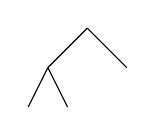
\begin{tikzpicture}
    [level distance=5mm,level/.style={sibling distance=10mm/#1}]
    \coordinate
      child {
        child {}
        child {}
      }
      child {};
  \end{tikzpicture} &
  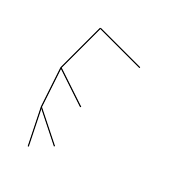
\begin{tikzpicture}
    [level distance=5mm,level/.style={sibling distance=10mm/#1}]
    \coordinate
      child {
        child {
          child {}
          child {}
        }
        child {}
      }
      child {};
  \end{tikzpicture} &
  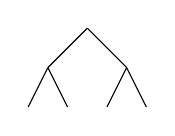
\begin{tikzpicture}
    [level distance=5mm,level/.style={sibling distance=10mm/#1}]
    \coordinate
      child {
        child {}
        child {}
      }
      child {
        child {}
        child {}
      };
  \end{tikzpicture} &
  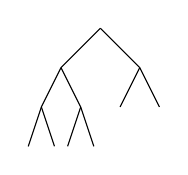
\begin{tikzpicture}
    [level distance=5mm,level/.style={sibling distance=10mm/#1}]
    \coordinate
      child {
        child {
          child {}
          child {}
        }
        child {
          child {}
          child {}
        }
      }
      child {
        child {}
        child {}
      };
  \end{tikzpicture} &
  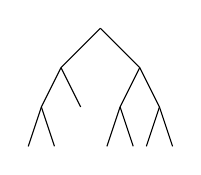
\begin{tikzpicture}
    [level distance=5mm,level/.style={sibling distance=10mm/#1}]
    \coordinate
      child {
        child {
          child {}
          child {}
        }
        child {}
      }
      child {
        child {
          child {}
          child {}
        }
        child {
          child {}
          child {}
        }
      };
  \end{tikzpicture} &
  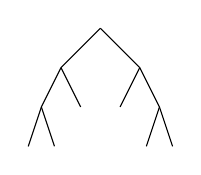
\begin{tikzpicture}
    [level distance=5mm,level/.style={sibling distance=10mm/#1}]
    \coordinate
      child {
        child {
          child {}
          child {}
        }
        child {}
      }
      child {
        child {}
        child {
          child {}
          child {}
        }
      };
  \end{tikzpicture} &
  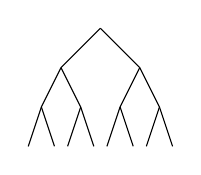
\begin{tikzpicture}
    [level distance=5mm,level/.style={sibling distance=10mm/#1}]
    \coordinate
      child {
        child {
          child {}
          child {}
        }
        child {
          child {}
          child {}
        }
      }
      child {
        child {
          child {}
          child {}
        }
        child {
          child {}
          child {}
        }
      };
  \end{tikzpicture} &
  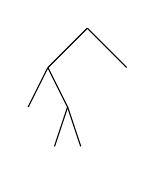
\begin{tikzpicture}
    [level distance=5mm,level/.style={sibling distance=10mm/#1}]
    \coordinate
      child {
        child {}
        child {
          child {}
          child {}
        }
      }
      child {};
  \end{tikzpicture} \\
  1 & 2 & 0 & 1 & 1 & 1 & 0 & 2 \\
\end{tabular}
\]
%
Razred \verb|Drevo| razširite z metodo \verb|naloga2(self)|, ki vrne neuravnoteženost podanega dvojiškega drevesa.
Me\-to\-da naj deluje v času $O(n)$, kjer je $n$ število vozlišč v drevesu.

%%%%%%%%%%%%%%%%%%%%%%%%%%%%%%%%%%%%%%%%%%%%%%%%%%%%%%%%%%%%%%%%%%%%%%
\naloga[30 točk]
Pri tej nalogi boste v \emph{Mathematici} risali grafe z vozlišči $v_1, \dots, v_n$,
enakomerno razporejenimi po krogu.
\emph{Razmik} med vozliščema $v_i$ in $v_j$ definiramo kot $|i - j| \bmod n$.

\podnaloga[20 točk]
V \emph{Mathematici} sestavite funkcijo \verb|naloga3a[n_, sez_]|, ki nariše graf
na \verb|n| vozliščih, pri čemer sta dve vozlišči povezani takrat,
kadar je njun razmik v seznamu \verb|sez|.

\begin{center}
  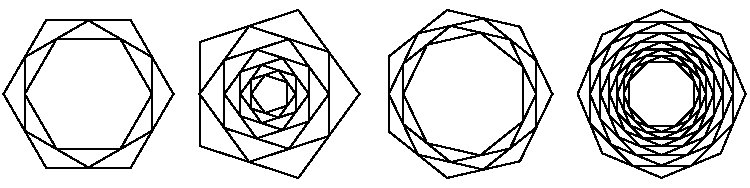
\includegraphics[width=\textwidth]{naloga3a.pdf} \\
  \hfill
  \verb|naloga3a[6,{1,2}]|\hfill
  \verb|naloga3a[7,{1,2}]|\hfill
  \verb|naloga3a[7,{3,5}]|\hfill
  \verb|naloga3a[8,{1,3,4}]|\hfill
\end{center}

\podnaloga[10 točk]
V \emph{Mathematici} sestavite funkcijo \verb|naloga3b[n_]|, ki nariše graf
na \verb|n| vozliščih, pri čemer sta dve vozlišči povezani takrat, kadar je njun razmik tuj številu \verb|n|.

\begin{center}
  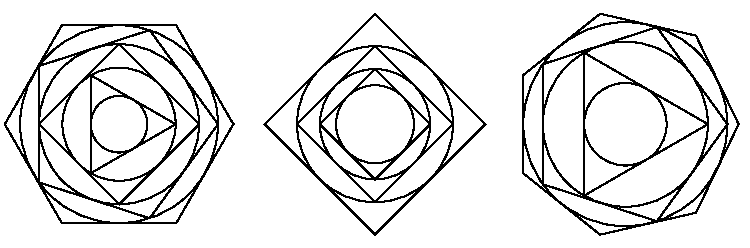
\includegraphics[width=\textwidth]{naloga3b.pdf} \\
  \verb|naloga3b[6]|\qquad\quad\qquad
  \verb|naloga3b[8]|\qquad\quad\qquad
  \verb|naloga3b[9]|\qquad\quad\qquad
  \verb|naloga3b[10]|
\end{center}

%%%%%%%%%%%%%%%%%%%%%%%%%%%%%%%%%%%%%%%%%%%%%%%%%%%%%%%%%%%%%%%%%%%%%%
\naloga[25 točk]

Podane naj bodo končne množice $A_1, A_2, \dots, A_n \subseteq \mathbb{N}$.
Na kartezičnem produktu $A_1 \times A_2 \times \dots \times A_n$ uvedemo leksikografsko ureditev $n$-teric.
Na primer, na produktu $\{1, 5, 9\} \times \{2, 4\} \times \{1, 4\}$ veljajo naslednje neenakosti:

\begin{align*}
  &(1, 2, 1) < (1, 2, 4) < (1, 4, 1) < (1, 4, 4) < (5, 2, 1) < (5, 2, 4) < \\
  &\ \ (5, 4, 1) < (5, 4, 4) < (9, 2, 1) < (9, 2, 4) < (9, 4, 1) < (9, 4, 4)
\end{align*}
%
Sestavite funkcijo \verb|naloga4(sez, k)|,
ki za seznam množic $\mathtt{sez} = [A_1, \dots, A_n]$
vrne \verb|k|-to $n$-terico glede na leksikografsko ureditev.
Funkcija naj deluje v času $O(n m \log m)$, kjer je $m$ velikost največje množice.
Če je \verb|k| manjši ali enak $0$ oziroma večji od velikosti kartezičnega produkta, naj funkcija vrne \verb|None|.

\begin{verbatim}
>>> naloga4([{1, 5, 9}, {2, 4}, {1, 4}], 1)
(1, 2, 1)
>>> naloga4([{1, 5, 9}, {2, 4}, {1, 4}], 7)
(5, 4, 1)
>>> naloga4([{1, 5, 9}, {2, 4}, {1, 4}], 12)
(9, 4, 4)
\end{verbatim}


\end{document}

